\chapter{Opis sustava i tehničkih zahtjeva}

\section{Opis problematike hrkanja kao zdravstvenog problema}

Hrkanje je čest poremećaj koji pogađa 20-40\% opće populacije. Ono nastaje kao posljedica vibracije anatomskih struktura u dišnom putu. Treperenje mekog nepca odgovorno je za grubi aspekt zvuka hrkanja. Na hrkanje utječu mnogi faktori kao što su položaj tijela, faza spavanja, dišni putevi i prisutnost ili odsutnost poremećaja disanja tijekom spavanja. Pojava hrkanja može varirati tijekom noći \cite{pevernagie}. 

Iako se hrkanje općenito doživljava kao društvena smetnja, ocjena njegove bučnosti subjektivna je i stoga nedosljedna. Objektivna procjena hrkanja važna je za procjenu učinka terapijskih intervencija. Štoviše, hrkanje nosi informacije koje se odnose na mjesto i stupanj opstrukcije gornjih dišnih putova.

\subsection{Anatomija i klasifikacija hrkanja}
Gornji dišni putovi su područje od nosnica i usana do glasnica. Sastoje se od nosne i usne šupljine, ždrijela i gornjeg dijela grkljana. Ždrijelo je stražnji dio glave i sadrži nekoliko anatomskih orijentira, kao što su meko nepce (velum), nepčani krajnici, korijen jezika i nepčana resica (epiglotis). Epiglotis odvaja ždrijelo od jednjaka i grkljana, koji sadrži glasnice \cite{snoringml}.

\begin{figure}[ht]
	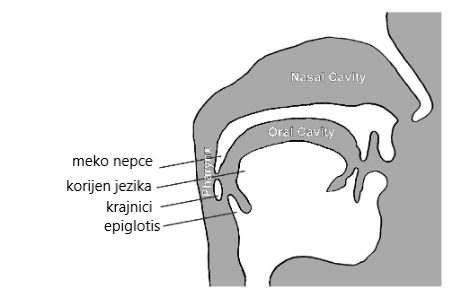
\includegraphics[width=\linewidth]{imgs/anatomy}
	\caption{Anatomija gornjih dišnih puteva \cite{snoringml}}
	\label{fig:anatomy}
\end{figure}

Hrkanje je uzrokovano vibracijama struktura mekog tkiva u gornjim dišnim putovima, osobito na fiziološkim suženjima. 
Tijekom sna, tonus mišića se smanjuje, a meko tkivo opušta, povećavajući njegovu sklonost vibriranju. Brzina protoka zraka pri udisaju povećava se u uskim dijelovima gornjih dišnih puteva, izazivajući vibracije tkiva i strujanja zraka, što zauzvrat uzrokuje hrkanje.

Tipična područja koja pridonose stvaranju zvuka hrkanja su meko nepce i njegov vrh, uvula, koja može vibrirati u anteriorno-posteriornom smjeru, nepčani krajnici koji obično vibriraju u lateralnom smjeru, korijen jezika koja može pasti natrag i ograničiti prolaz prema stražnjoj stijenci ždrijela i epiglotis, koji se može spustiti zbog smanjene strukturne krutosti ili zbog stražnjeg pomaka prema stražnjoj stijenci ždrijela.

Za ciljano liječenje hrkanja i srodnih poremećaja disanja povezanih sa spavanjem, ključno je identificirati mehanizme i mjesta koja doprinose sužavanju dišnih puteva i uzrokuju hrkanje ili respiratorne opstrukcije kod pojedinog subjekta.

%\subsection{Klasifikacija hrkanja}

Široko korištena definicija raznih mehanizama hrkanja je VOTE klasifikacija, koja razlikuje četiri razine u kojima se mogu pojaviti hrkanje i sužavanje dišnih puteva:
\begin{itemize}
	\item V - \textit{Velum}: razina mekog nepca, 
	\item O - \textit{Oropharynx}: razina usnog dijela ždrijela,  
	\item T - \textit{Tongue}: razina korijena jezika, 
	\item E - \textit{Epiglottis}: razina epiglotisa. 
\end{itemize}

U radu \cite{bib} uspoređeni su zvukovi hrkanja izazvani tijekom nazendoskopije s onima u prirodnom snu pomoću spektra zvučnih frekvencija. Pacijenti s palatinalnim hrkanjem tijekom nazendoskopije u snu imali su srednju vršnu frekvenciju od 137 Hz. Najveća frekvencija hrkanja u korijenu jezika bila je 1243 Hz, a kombinirano hrkanje nepca i jezika 190 Hz. Središnje frekvencije bile su 371, 1094 i 404 Hz. Epiglotično hrkanje imalo je vršnu frekvenciju od 490 Hz. Iako rezultati pokazuju da inducirano hrkanje sadrži komponentu više frekvencije zvuka koja nije vidljiva tijekom prirodnog hrkanja, korelacija je dovoljno dobra za kategoriziranje zvučnih zapisa hrkanja. 

Također, visina zvuka hrkanja u niskofrekventnom rasponu (<500 Hz) odgovara osnovnoj frekvenciji s pripadajućim harmonicima. Visina hrkanja određena je vibracijom mekog nepca, dok je nepalatalno hrkanje više „nalik buci“ i ima raspršeniju energiju u višim spektralnim podpojasevima (>500 Hz).


\section{Zahtjevi na sustav i opis predloženog rješenja}

Sustav se mora sastojati od dva fizička dijela, odnosno računala i mikrokontrolera. Odabrani mikrokontroler treba sadržavati mikrofon koji može primati audio signal iz svih smjerova. Mikrofon mora primati zvuk na udaljenosti barem jedan metar, stoga je potrebno analizirati ovisnost udaljenosti i intenziteta zvuka snimanjem zvučnih zapisa odabranim hardverom. Isto tako, hardver mora podržavati bežično povezivanje i slanje podataka na računalo. Bežični prijenos treba biti ostvaren BLE sučeljem. Računalna aplikacija mora podržavati prijam podataka putem BLE sučelja te omogućiti njihovu pohranu. Također, mora imati razvijeno grafičko korisničko sučelje putem kojeg se može komunicirati s odabranim mikrokontrolerom, točnije moći pokrenuti snimanje zvuka.

U okviru ovog završnog rada razvijena je programska potpora za mikrokontroler \newline STM32WB5M te je uspostavljeno BLE komunikacijsko sučelje između razvojnog sustava i osobnog računala s operacijskim sustavom Linux. Sučeljem se prenosi zvučni signal sniman MEMS mikrofonom s mikrokontrolera na računalo. Također je i razvijeno korisničko sučelje za pokretanje komunikacije, prijam i pohranu signala. Blok shema sustava prikazana je na slici \ref{fig:shema}. 

\begin{figure}[ht]
	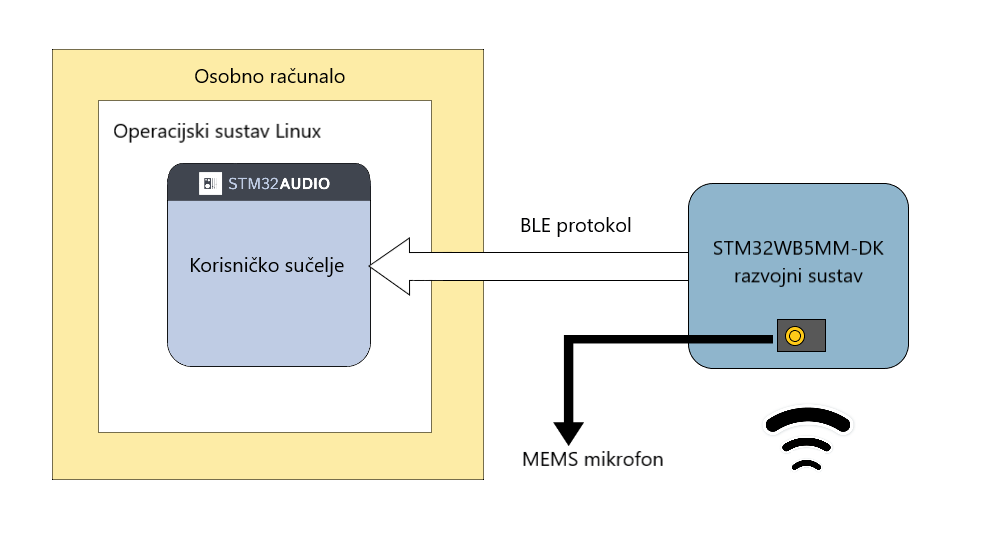
\includegraphics[width=\linewidth]{imgs/shema}
	\caption{Blok shema sustava}
	\label{fig:shema}
\end{figure}

